%\usepackage{ucs}
%\usepackage{pb-diagram}
%\usepackage{epstopdf}
%\usepackage{verbatim}
%\newenvironment{comment}
%{\par\noindent{\bf TODO}\\}
%{\\\hfill$\scriptstyle\blacksquare$\par}


\documentclass[12pt]{article}
\usepackage{amssymb}

%%%%%%%%%%%%%%%%%%%%%%%%%%%%%%%%%%%%%%%%%%%%%%%%%%%%%%%%%%%%%%%%%%%%%%%%%%%%%%%%%%%%%%%%%%%%%%%%%%%%
\usepackage{amsmath}
\usepackage{amsmath,amssymb,amsthm}
\usepackage{multicol}
\usepackage{color}
\usepackage{graphicx}
\usepackage{hyperref}

%TCIDATA{OutputFilter=Latex.dll}
%TCIDATA{LastRevised=Wed Dec 15 21:36:06 2010}
%TCIDATA{<META NAME="GraphicsSave" CONTENT="32">}
%TCIDATA{CSTFile=article.cst}

\newtheorem{statement}{Statement}
\newtheorem{theorem}{Theorem}
\newtheorem{corollary}{Corollary}[theorem]
\newtheorem{lemma}{Lemma}
\newtheorem{mynote}{Note}[section]
%\newtheorem{proof}{Proof}
\theoremstyle{definition}
\newtheorem{definition}{Definition}
\newtheorem{remark}{Remark}
\newtheorem{example}{Example}
\newcommand{\go}{\stackrel{\circ }{\mathfrak{g}}}
\newcommand{\ao}{\stackrel{\circ }{\mathfrak{a}}}
\newcommand{\co}[1]{\stackrel{\circ }{#1}}
\newcommand{\pia}{\pi_{\mathfrak{a}}}
\newcommand{\piab}{\pi_{\mathfrak{a}_{\bot}}}
\newcommand{\gf}{\mathfrak{g}}
\newcommand{\af}{\mathfrak{a}}
\newcommand{\aft}{\widetilde{\mathfrak{a}}}
\newcommand{\afb}{\mathfrak{a}_{\bot}}
\newcommand{\hf}{\mathfrak{h}}
\newcommand{\hfb}{\mathfrak{h}_{\bot}}
\newcommand{\pf}{\mathfrak{p}}
%\input{tcilatex}

\begin{document}

\title{Recursive properties of branching and Weyl-Verma formulas}
\author{V D Lyakhovsky$^1$ and A A Nazarov$^2$}

\maketitle

\begin{abstract}
Recurrent relations for branching coefficients are based on a special type of
singular element decomposition. We show that this decomposition can be used to
construct the parabolic Verma modules and finally to obtain the generalized
Weyl-Verma formulas for characters.
These Weyl-Verma formulas explicitly exhibit how branching and the generalized
BGG-resolution properties are connected.
\end{abstract}



\section{Introduction}

\label{sec:introduction}

Branching properties of Lie (affine Lie) algebras are highly important for
applications in quantum field theory (see for example the conformal field
theory models \cite{difrancesco1997cft},\cite{coquereaux2008conformal}). In
this paper we demonstrate that for an arbitrary reductive subalgebra
branching is directly connected with the BGG resolution and in particular
exhibits the resolution properties in terms of the $\mathcal{O}^{p}$
category \cite{lepowsky1977generalization} (the parabolic generalization of
the cathegory $\mathcal{O}$ \cite{bernstein1976category}).

The resolution of the irreducible modules in terms of infinite-dimensional ones is important for the
theory of integrable spin chains \cite{derk1008}. In the Baxter $\mathcal{Q}$-operator approach the generic transfer
matrices corresponding to the (generalized) Verma modules are factorized into the product of Baxter
operator. Then the resolution allows to calculate the transfer matrices for finite-dimensional
auxiliary spaces. 

To show the connection of the BGG resolution with the branching we use the recursive approach presented in \cite
{2010arXiv1007.0318L} (similar to the one used in \cite{ilyin812pbc} for
maximal embeddings). We consider the subalgebra $\af$ together with its
counterpart $\afb$ ''orthogonal'' to $\af$ with respect to
the Killing form and also $\widetilde{\afb}:=\afb\oplus \frak{h}_{\perp }$ where $\frak{h}=\frak{\frak{h}_{\af}}\oplus
\frak{h}_{\afb}\oplus \frak{h}_{\perp }$. For any reductive
algebra $\af$ the subalgebra $\afb\hookrightarrow \gf$
is regular and reductive. For a highest weight integrable module $%
L^{\left(\mu \right) }$ and orthogonal subalgebra $\af_{\bot }$ we
consider the singular element $\Psi ^{\left( \mu \right) }$ (the numerator
in the Weyl character formula $ch\left( L^{\mu }\right) =\frac{\Psi ^{\left(
\mu \right) }}{\Psi ^{\left( 0\right) }}$, see for example \cite
{humphreys1997introduction}) the Weyl denominator $\Psi _{\af_{\bot
}}^{\left( 0\right) }$ for the orthogonal subalgebra and the projection $%
\Psi _{\left( \af,\af_{\bot }\right) }^{\left( \mu \right) }=\pi _{%
\af}\frac{\Psi _{\gf}^{\left( \mu \right) }}{\Psi _{\af_{\bot
}}^{\left( 0\right) }}$. It is shown that the element $\Psi _{\gf%
}^{\left( \mu \right) }$ can be decomposed into a combination of Weyl
numerators $\Psi _{\af_{\bot }}^{\left( \nu \right) }$ with $\nu \in P_{%
\mathfrak{a}_{\bot}}^{+}$. This decomposition provides the possibility to
construct the set of highest weight modules $L_{\widetilde{\afb}%
}^{\mu _{\widetilde{\afb}}}$. When the injection \ $\af%
_{\bot }\hookrightarrow \gf$ \ satisfies the ''standard parabolic''
conditions these modules give rise to the parabolic Verma modules $M_{\left(
\widetilde{\afb}\hookrightarrow \gf\right) }^{\mu _{%
\widetilde{\afb}}}$ so that the initial character $ch\left(
L^{\mu }\right) $ is finally decomposed into the alternating sum of such. On
the other hand when the parabolic conditions are violated the construction
survives and exhibits a decomposition with respect to a set of Verma
modules $M_{\left( \widetilde{\frak{b}_{\perp }},\gf\right) }^{\mu _{%
\widetilde{\afb}}}$. In such a situation the algebra $%
\widetilde{\frak{b}_{\perp }}$ is not a subalgebra in $\gf$ but a
contraction of $\widetilde{\afb}$.

Some general properties of the proposed decompositions are formulated in
terms of a specific element $\Gamma _{\af\rightarrow \gf}$ of the
group algebra $\mathcal{E}\left( \gf\right) $ called ''the injection
fan''. Using this tool the simple and explicit algorithm for branching
coefficients computations applicable for an arbitrary (maximal or
nonmaximal) subalgebras of finite-dimensional or affine Lie algebras was
obtained in \cite{2010arXiv1007.0318L}.

Possible further developments are presented in Section \ref{sec:conclusions}.

\subsection{Notation}

\label{sec:notation}

Consider Lie algebras (affine Lie algebras) $\gf$ and $\af$ and an
injection $\af\hookrightarrow \gf$ such that $\af$ is a
reductive subalgebra $\frak{a\subset g}$ with correlated root spaces: $\frak{%
h}_{\af}^{\ast }\subset \frak{h}_{\gf}^{\ast }$. We use the
following notations:

$\frak{g=n}^{-}+\frak{b}+\frak{n}^{+}$ --- the Cartan decomposition;

$r$ , $\left( r_{\af}\right) $ --- the rank of the algebra $\gf$ $%
\left( \mathrm{{resp. }\af}\right) $ ;

$\Delta $ $\left( \Delta _{\af}\right) $--- the root system; $\Delta
^{+} $ $\left( \mathrm{{resp. }\Delta _{\af}^{+}}\right) $--- the
positive root system (of $\gf$ and $\af$ respectively);

$\mathrm{mult}\left( \alpha \right) $ $\left( \mathrm{mult}_{\af}\left(
\alpha \right) \right) $ --- the multiplicity of the root $\alpha$ in $%
\Delta $ (resp. in $\left( \Delta _{\af}\right) $);

$S\quad \left( S_{\af}\right) $ --- the system of simple roots (of $%
\gf$ and $\af$ respectively);

$\alpha _{i}$ , $\left( \alpha _{\left( \af\right) j}\right) $ --- the $%
i$-th (resp. $j$-th) basic root for $\gf$ $\left( \mathrm{{resp.}\frak{a%
}}\right) $; $i=0,\ldots ,r$,\ \ $\left( j=0,\ldots ,r_{\af}\right) $;

$\delta $ --- the imaginary root of $\gf$ (and of $\af$ if any);

$\alpha _{i}^{\vee }$ , $\left( \alpha _{\left( \af\right) j}^{\vee
}\right) $--- the basic coroot for $\gf$ $\left( \mathrm{{resp.}\af%
}\right) $ , $i=0,\ldots ,r$ ;\ \ $\left( j=0,\ldots ,r_{\af}\right) $;

$W$ , $\left( W_{\af}\right) $--- the corresponding Weyl group;

$C$ , $\left( C_{\af}\right) $--- the fundamental Weyl chamber;

$\bar{C}, \left(\bar{C_{\af}}\right)$ --- the closure of the
fundamental Weyl chamber;

$\epsilon \left( w\right) :=\left( -1\right) ^{\mathrm{length}(w)}$;

$\rho $\ , $\left( \rho _{\af}\right) $\ --- the Weyl vector;

$L^{\mu }$\ $\left( L_{\af}^{\nu }\right) $\ --- the integrable module
of $\gf$ with the highest weight $\mu $\ ; (resp. integrable $\af$
-module with the highest weight $\nu $ );

$\mathcal{N}^{\mu }$ , $\left( \mathcal{N}_{\af}^{\nu }\right) $ ---
the weight diagram of $L^{\mu }$ (resp. ${}L_{\af}^{\nu }$ );

$P$ (resp. $P_{\af} $) \ --- the weight lattice;

$P^{+}$ (resp. $P_{\af}^{+} $) \ --- the dominant weight lattice;

$m_{\xi }^{\left( \mu \right) }$ , $\left( m_{\xi }^{\left( \nu \right)
}\right) $ --- the multiplicity of the weight $\xi \in P$ \ $\left( \mathrm{{%
resp. }\in P_{\af}}\right) $ in the module $L^{\mu }$ , (resp. $\xi \in
L_{\af}^{\nu } $);

$ch\left( L^{\mu }\right) $ (resp. $\mathrm{ch}\left( L_{\af}^{\nu
}\right) $)--- the formal character of $L^{\mu }$ (resp. $L_{\af}^{\nu
} $);

$ch\left( L^{\mu }\right) =\frac{\sum_{w\in W}\epsilon (w)e^{w\circ (\mu
+\rho )-\rho }}{\prod_{\alpha \in \Delta ^{+}}\left( 1-e^{-\alpha }\right) ^{%
\mathrm{{mult}\left( \alpha \right) }}}$ --- the Weyl-Kac formula;

$R:=\prod_{\alpha \in \Delta ^{+}}\left( 1-e^{-\alpha }\right) ^{\mathrm{{%
mult}\left( \alpha \right) }}\quad $ (resp. $R_{\af}:=\prod_{\alpha \in
\Delta _{\af}^{+}}\left( 1-e^{-\alpha }\right) ^{\mathrm{mult}_{\af%
}\left( \alpha \right) } $)--- the Weyl denominator.

\section{Orthogonal subalgebra and singular elements}

\label{sec:recurr-form-branch}

In this section we shall show how the recurrent approach to branching
problem leads naturally to a presentation of the formal character in terms
of parabolic (generalized) Verma modules. Consider a reductive Lie algebra $%
\gf$ and its reductive subalgebra $\af\subset \gf$. Let $%
L^{\mu} $ be the highest weight integrable module of $\gf$, $\mu \in
P^{+}$. Let $L^{\mu }$ be completely reducible with respect to $\af$,
\begin{equation*}
L_{\gf\downarrow \af}^{\mu }=\bigoplus\limits_{\nu \in P_{\af%
}^{+}}b_{\nu }^{\left( \mu \right) }L_{\af}^{\nu }.
\end{equation*}
Using the projection operator $\pi _{\af}$ (to the weight space $\frak{%
h_{a}}^{\ast }$) one can rewrite this decomposition in terms of formal
characters:
\begin{equation}
\pi _{\af}ch\left( L^{\mu }\right) =\sum_{\nu \in P_{\af%
}^{+}}b_{\nu }^{(\mu )}ch\left( L_{\af}^{\nu }\right) .
\label{branching1}
\end{equation}
The module $L^{\mu }$ has the BGG-resolution (see \cite
{bernstein1976category,bernstein1975differential,bernstein1971structure} and
\cite{humphreys2008representations}). All the members of the filtration
sequence are the direct sums of Verma modules and all their highest weights $%
\nu $ are strongly linked to $\mu $:
\begin{equation*}
\left\{ \nu \right\} =\left\{ w\left( \mu +\rho \right) -\rho |w\in
W\right\} .
\end{equation*}

\subsection{Orthogonal subalgebra}

Let $\frak{h}_{\af}$ be a Cartan subalgebra of $\mathfrak{g}$. For $%
\mathfrak{a}\hookrightarrow \gf$ introduce the ''orthogonal partner'' $%
\mathfrak{a}_{\bot }\hookrightarrow \gf$ .

Consider the root subspace $\frak{h}_{\perp \af}^{\ast }$ orthogonal to
$\af$,
\begin{equation*}
\frak{h}_{\perp \af}^{\ast }:=\left\{ \eta \in \frak{h}^{\ast }|\forall
h\in \frak{h}_{\af};\eta \left( h\right) =0\right\} ,
\end{equation*}
and the roots (correspondingly -- positive roots) of $\gf$ orthogonal
to $\af$,
\begin{eqnarray}
\Delta _{\afb} &:&=\left\{ \beta \in \Delta _{\gf}|\forall
h\in \frak{h}_{\af};\beta \left( h\right) =0\right\} ,
\label{delta a ort} \\
\Delta _{\afb}^{+} &:&=\left\{ \beta ^{+}\in \Delta _{\gf%
}^{+}|\forall h\in \frak{h}_{\af};\beta ^{+}\left( h\right) =0\right\} .
\notag
\end{eqnarray}
Let $W_{\afb}$ be the subgroup of $W$ generated by the
reflections $w_{\beta }$ with the roots $\beta \in \Delta _{\afb}^{+}$ . The subsystem $\Delta _{\afb}$ determines the
subalgebra $\afb$ with the Cartan subalgebra $\frak{h}_{\af%
_{\perp }}$. Let
\begin{equation*}
\frak{h}_{\perp }^{\ast }:=\left\{ \eta \in \frak{h}_{\perp \af}^{\ast
}|\forall h\in \frak{h}_{\af\oplus \afb};\eta \left(
h\right) =0\right\}
\end{equation*}
so that $\gf$ has the subalgebras
\begin{eqnarray*}
\widetilde{\afb} &:&=\afb\oplus \frak{h}_{\perp }
\\
\widetilde{\af} &:&=\af\oplus \frak{h}_{\perp }.
\end{eqnarray*}
Notice that $\mathfrak{a} \oplus \mathfrak{a}_{\bot}$ in general is not a
subalgebra of $\mathfrak{g}$

For the Cartan subalgebras we have the decomposition
\begin{equation}
\frak{h}=\frak{\frak{h}_{\af}}\oplus \frak{h}_{\afb}\oplus
\frak{h}_{\perp }=\frak{\frak{h}_{\widetilde{\af}}}\oplus \frak{h}_{%
\afb}=\frak{\frak{h}_{\widetilde{\afb}}}\oplus
\frak{h}_{\af}.
\end{equation}
For the subalgebras $\af$ and $\afb$ consider the
corresponding Weyl vectors, $\rho _{\af}$ and $\rho _{\afb} $ . Form the so called ''defects'' $\mathcal{D}_{\af}$ and $\mathcal{%
D}_{\afb}$ of the injection:
\begin{equation}
\mathcal{D}_{\af}:=\rho _{\af}-\pi _{\af}\rho ,
\end{equation}
\begin{equation}
\mathcal{D}_{\afb}:=\rho _{\afb}-\pi _{\af%
_{\perp }}\rho .  \label{defect ort}
\end{equation}

For the highest weight $\mu \in P^{+}$ consider the linked weights $\left\{
\left( w(\mu +\rho )-\rho \right) |w\in W\right\} $ and their projections to
$h_{\afb}^{\ast }$ additionally shifted by the defect $-%
\mathcal{D}_{\afb}$:
\begin{equation*}
\mu _{\afb}\left( w\right) :=\pi _{\afb}\left[
w(\mu +\rho )-\rho \right] -\mathcal{D}_{\afb},\quad w\in W.
\end{equation*}
For $\mu \in P^{+}$ among the weights $\left\{ \mu _{\afb}\left( w\right) |w\in W\right\} $ one can always choose those located in
the fundamental chamber $\overline{C_{\afb}}$. Let $U$ be the
set of representatives $u$ for the classes $W/W_{\afb}$ such
that

\begin{equation}
U:=\left\{ u\in W|\quad \mu _{\afb}\left( u\right) \in
\overline{C_{\afb}}\right\} \quad .  \label{U-def}
\end{equation}
Thus we can select the following subsets:
\begin{equation}
\mu _{\widetilde{\mathfrak{a}}}\left( u\right) :=\pi _{\widetilde{%
\mathfrak{a}}}\left[ u(\mu +\rho )-\rho \right] +\mathcal{D}_{\af%
_{\perp }},\quad u\in U,  \label{mu-a}
\end{equation}
and
\begin{equation}
\mu _{\afb}\left( u\right) :=\pi _{\afb}\left[
u(\mu +\rho )-\rho \right] -\mathcal{D}_{\afb},\quad u\in U.
\label{mu-a-tilda}
\end{equation}

Note that the subalgebra $\mathfrak{a}_{\bot}$ is regular by definition
since it is built on the roots of the algebra $\mathfrak{g}$.

For the modules we are interested in the Weyl-Kac formula for $\mathrm{ch}%
\left( L^{\mu }\right) $ can be written in terms of singular elements \cite
{humphreys1997introduction}
\begin{equation*}
\Psi ^{\left( \mu \right) }:=\sum\limits_{w\in W}\epsilon (w)e^{w(\mu +\rho
)-\rho },
\end{equation*}
namely,
\begin{equation}
\mathrm{ch}\left( L^{\mu }\right) =\frac{\Psi ^{\left( \mu \right) }}{\Psi
^{\left( 0\right) }}=\frac{\Psi ^{\left( \mu \right) }}{R}.
\label{Weyl-Kac2}
\end{equation}
The same is true for the submodules $\mathrm{ch}\left( L_{\af}^{\nu
}\right) $ in (\ref{branching1})
\begin{equation*}
\mathrm{ch}\left( L_{\af}^{\nu }\right) =\frac{\Psi _{\af}^{\left(
\nu \right) }}{\Psi _{\af}^{\left( 0\right) }}=\frac{\Psi _{\af%
}^{\left( \nu \right) }}{R_{\af}},
\end{equation*}
with
\begin{equation*}
\Psi _{\af}^{\left( \nu \right) }:=\sum\limits_{w\in W_{\af%
}}\epsilon (w)e^{w(\nu +\rho _{_{\af}})-\rho _{_{\af}}}.
\end{equation*}

Applying formula (\ref{Weyl-Kac2}) to the branching rule (\ref{branching1})
we get the relation connecting the singular elements $\Psi ^{\left( \mu
\right) }$ and $\Psi _{\af}^{\left( \nu \right) }$ :
\begin{eqnarray}
\pi _{\af}\left( \frac{\sum_{w \in W}\epsilon (w )e^{w (\mu +\rho
)-\rho }}{\prod_{\alpha \in \Delta ^{+}}(1-e^{-\alpha })^{\mathrm{mult}%
(\alpha )}}\right) &=&\sum_{\nu \in P_{\af}^{+}}b_{\nu }^{(\mu )}\frac{%
\sum_{w \in W_{\af}}\epsilon (w )e^{w (\nu +\rho _{\af})-\rho _{%
\af}}}{\prod_{\beta \in \Delta _{\af}^{+}}(1-e^{-\beta })^{\mathrm{%
mult}_{\af}(\beta )}},  \notag  \label{eq:4} \\
\pi _{\af}\left( \frac{\Psi ^{\left( \mu \right) }}{R}\right)
&=&\sum_{\nu \in P_{\af}^{+}}b_{\nu }^{(\mu )}\frac{\Psi _{\af%
}^{\left( \nu \right) }}{R_{\af}}.
\end{eqnarray}

\subsection{Decomposing the singular element.}

\label{subsec:decomp-sing-element}

Now we shall perform a decomposition of the singular element $\Psi ^{\left(
\mu \right) }$ in terms of singular elements of the orthogonal subalgebra
modules:

\begin{lemma}
Let $\af_{\bot }$ be the orthogonal partner of a reductive subalgebra $%
\af\hookrightarrow \gf$ with $\frak{h}=\frak{\frak{h}_{\af}}%
\oplus \frak{h}_{\afb}\oplus \frak{h}_{\perp }$, $\widetilde{%
\afb}=\afb\oplus \frak{h}_{\perp }$ and $%
\widetilde{\af}=\af\oplus \frak{h}_{\perp }$.

$L^{\mu }$ be the highest weight integrable module with $\mu \in P^{+}$ and

$\Psi ^{\left( \mu \right) }$\ -- the singular element of $L^{\mu }$.

Then the element $\Psi ^{\left( \mu \right) }$ can be decomposed into the
sum over $u\in U$ (see (\ref{U-def})) of singular elements $\Psi _{\af%
_{\perp }}^{\mu _{\afb}\left( u\right) }$ with the coefficients
$\epsilon (u)e^{\mu _{\widetilde{\mathfrak{a}}}\left( u\right) }$:
\begin{equation}
\Psi ^{\left( \mu \right) }=\sum_{u\in U}\;\epsilon (u)e^{\mu _{\widetilde{%
\mathfrak{a}}}\left( u\right) }\Psi _{\afb}^{\mu _{\af%
_{\perp }}\left( u\right) }.  \label{sing decomp main}
\end{equation}
\end{lemma}

\begin{proof}
With $u\in U$ and $v\in W_{\af_{\bot }}$ perform the decomposition
\[
u(\mu +\rho )=\pi _{\left( \aft\right) }u(\mu +\rho )+\pi _{\left(
\afb\right) }u(\mu +\rho )
\]
for the singular weight $vu(\mu +\rho )-\rho $:
\begin{equation}
\begin{array}{lcl}
vu(\mu +\rho )-\rho  & = & \pi _{\left( \af\right) }\left( u(\mu +\rho
)\right) -\rho +\rho _{\afb}
\\
&  & +\ v\left( \pi _{\left( \aft_{\perp }\right) }u(\mu
+\rho )-\rho _{\afb}+\rho _{\afb}\right) -\rho _{%
\afb} .
\end{array}
\label{sing-decomp-1}
\end{equation}
Use the defect $\mathcal{D}_{\af_{\bot }}$ (\ref{defect ort}) to
simplify the first line in (\ref{sing-decomp-1}):
\[
\begin{array}{r}
\pi _{\left( \aft\right) }\left( u(\mu +\rho )\right) -\rho +\rho _{%
\afb}= \\
\pi _{\left( \aft\right) }\left( u(\mu +\rho )\right) -\pi _{\aft%
}\rho -\pi _{\af_{\bot }}\rho +\rho _{\af_{\bot }}= \\
=\pi _{\left( \aft\right) }\left( u(\mu +\rho )-\rho \right) +\mathcal{D}%
_{\af_{\bot }},
\end{array}
\]
and the second one:
\[
\begin{array}{c}
v\left( \pi _{\left( \afb\right) }u(\mu +\rho
)-\rho _{\afb}+\rho _{\afb}\right) -\rho _{\af%
_{\perp }}= \\
v\left( \pi _{\left( \af_{\bot }\right) }u(\mu +\rho )-%
\mathcal{D}_{\af_{\bot }}-\pi _{\left( \af_{\bot }\right) }\rho
+\rho _{\af_{\bot }}\right)
-\rho _{\af_{\bot }}= \\
=v\left( \pi _{\left( \af_{\bot }\right) }\left[ u(\mu
+\rho )-\rho \right] -\mathcal{D}_{\af_{\bot }}+\rho _{\af_{\bot
}}\right) -\rho _{\af_{\bot }}.
\end{array}
\]
These expressions provide the desired decomposition of the singular element $%
\Psi ^{\mu }$ in terms of singular elements $\Psi _{\af%
_{\perp }}^{\eta }$ of the $\afb$-modules $L_{%
\afb}^{\eta }$:
\begin{equation}
\begin{array}{l}
\Psi ^{\mu }=\sum_{u\in U}\sum_{v\in W_{\afb}}\epsilon
(v)\epsilon (u)e^{vu(\mu +\rho )-\rho }= \\
=\sum_{u\in U}\epsilon (u)e^{\pi _{\aft}\left[ u(\mu +\rho )-\rho \right]
+\mathcal{D}_{\afb}}\sum_{v\in W_{\afb}}\epsilon
(v)e^{v\left( \pi _{\left( \afb\right) }\left[
u(\mu +\rho )-\rho \right] -\mathcal{D}_{\afb}+\rho _{\af%
_{\perp }}\right) -\rho _{\afb}}= \\
=\sum_{u\in U}\;\epsilon (u)\Psi _{\afb}^{\pi
_{\left( \afb\right) }\left[ u(\mu +\rho )-\rho
\right] -\mathcal{D}_{\afb}}e^{\pi _{\left( \aft\right) }%
\left[ u(\mu +\rho )-\rho \right] +\mathcal{D}_{\afb}}.
\end{array}
\label{singular main}
\end{equation}
\end{proof}

\bigskip

\begin{remark}
This relation can be considered as a generalized form of the Weyl formula
for the singular element $\Psi _{\gf}^{\mu }$: the vectors $\mu _{%
\widetilde{\mathfrak{a}}}\left( u\right) $ play the role of singular weights
while the alternating factors $\epsilon (u)$ are extended to $\epsilon
(u)\Psi _{\afb}^{\mu _{\afb}\left( u\right) }$. In
fact when $\frak{a=g}$ both $\afb$and $\frak{h}_{\perp }$are
zeros, $U=W$, and\ the original Weyl formula is reobtained via the
trivilization of the singular elements: $\epsilon (u)\Psi _{\afb}^{\mu _{\afb}\left( u\right) }=\epsilon (u)$. In the opposite
limit when $\frak{a=0}$, $\Delta _{\afb}=\Delta _{\gf}$, $%
\frak{h}_{\perp }^{\ast }=0$, $\afb=\gf$, $\mathcal{D}_{%
\afb}=0$, $U=W/W_{\afb}=e$ and $\Psi ^{\mu }$ is
again reobtained, now via the trivilization of the set of vectors: $\mu _{%
\af}\left( e\right) =0$.
\end{remark}

\subsection{Reduction of Verma modules}

In \cite{2010arXiv1007.0318L} the decomposition analogous to (\ref{singular main}) was
used to construct the recurrent relations for branching coefficients $k_{\xi
}^{\left( \mu \right) }$ corresponding to the injection $\af%
\hookrightarrow \gf$:
\begin{equation}
\begin{array}{c}
k_{\xi }^{\left( \mu \right) }=-\frac{1}{s\left( \gamma _{0}\right) }\left(
\sum_{u\in U}\epsilon (u)\;\dim \left( L_{\afb}^{\mu _{\af%
_{\perp }}\left( u\right) }\right) \delta _{\xi -\gamma _{0},\pi _{\af%
}(u(\mu +\rho )-\rho )}+\right.  \\
\left. +\sum_{\gamma \in \Gamma _{\af\rightarrow \gf}}s\left(
\gamma +\gamma _{0}\right) k_{\xi +\gamma }^{\left( \mu \right) }\right) .
\end{array}
\label{recurrent rel}
\end{equation}
The recursion is goverened by the set $\Gamma _{\af\rightarrow \gf}
$ called the injection fan. The later is defined as the carrier set $\left\{
\xi \right\} _{\af\rightarrow \gf}$ for the coefficient function $%
s(\xi )$
\begin{equation*}
\left\{ \xi \right\} _{\af\rightarrow \gf}:=\left\{ \xi \in P_{%
\af}|s(\xi )\neq 0\right\}
\end{equation*}
appearing in the expansion
\begin{equation}
\prod_{\alpha \in \Delta ^{+}\setminus \Delta _{\afb }^{+}}\left( 1-e^{-\pi
_{\af}\alpha }\right) ^{\mathrm{mult}(\alpha )-\mathrm{mult}_{\af%
}(\pi _{\af}\alpha )}=-\sum_{\gamma \in P_{\af}}s(\gamma
)e^{-\gamma };\quad
\end{equation}
The weights in $\left\{ \xi \right\} _{\af\rightarrow \gf}$ are to
be shifted by $\gamma _{0}$ -- the lowest vector in $\left\{ \xi \right\} $
-- and the zero element is to be eliminated:
\begin{equation}
\Gamma _{\af\rightarrow \gf}=\left\{ \xi -\gamma _{0}|\xi \in
\left\{ \xi \right\} \right\} \setminus \left\{ 0\right\} .
\end{equation}

The recursion relation (\ref{recurrent rel}) was originally used to
described branchings for integrable modules. There exists an important class
of modules that also can be reduced with the help of an injection fan --
these are the Verma modules.

For a regular embedding $\af\hookrightarrow \gf$ we have the
corresponding embedding for the root systems $\Delta _{\mathfrak{a}%
}^{+}\hookrightarrow \Delta ^{+}$ . Moreover, in this case it is reasonable
to enlarge the subalgebra $\af$ and consider $\frak{b}=\af\oplus
\frak{h}_{\perp \af}$ . In this case the weights of a $\frak{b}$-module
can be considered in $\frak{h}^{\ast }$ . Verma module is decomposable for
any highest weight:
\begin{equation}
\mathrm{ch}M^{\mu }=\sum_{\nu }b_{\nu }^{(\mu )}\mathrm{ch}M_{\frak{b}}^{\nu
}.
\end{equation}
Verma module $\mathrm{ch}M^{\mu }$ have one singular weight $\mu $ with the
multiplicity ($+1$). The Weyl groups can be considered to be trivial. The
orthogonal partner $\afb$ is also trivial and the recursion
relation is simplified:
\begin{equation*}
k_{\xi }^{\left( \mu \right) }=-\frac{1}{s\left( \gamma _{0}\right) }%
\;\left( \delta _{\xi -\gamma _{0},\mu }+\sum_{\gamma \in \Gamma _{\af%
\rightarrow \gf}}s\left( \gamma +\gamma _{0}\right) k_{\xi +\gamma
}^{\left( \mu \right) }\right) .
\end{equation*}

\begin{remark}
Notice that inside the main Weyl chamber branching coefficients $k_{\xi
}^{\left( \mu \right) }$ for Verma modules reduction coincide with the
coefficients for reduction of integrable simple modules.
\end{remark}

\begin{example}
\label{example:reduct-verma-modul}
 Let $\mathfrak{g}=B_{2}$ be and consider $A_{1}=\mathfrak{a}%
\hookrightarrow \mathfrak{g}$. There are different embeddings  $%
A_{1}\hookrightarrow B_{2}$. Here we limit ourselves by the regular ones.
The root system $\Delta _{B_{2}}$ consists of 8 roots. Let $%
S_{B_{2}}=\left\{ \alpha _{1}=e_{1}-e_{2},\alpha _{2}=e_{2}\right\} $ where $%
e_{1},e_{2}$ form the standard basis in $\mathbf{R}^{2}$. The set of the
positive roots is $\Delta ^{+}=\left\{ \alpha _{1},\alpha _{1}+\alpha
_{2},\alpha _{1}+2\alpha _{2},\alpha _{2}\right\} $. Each of these roots can
be taken as the simple root of the $A_{1}-$subalgebra. Firstly  we consider
the subalgebra $A_{1}$ with the simple root $\beta =\alpha _{1}+2\alpha _{2}$%
. Consider the Verma module $M^{\mu }$ with the highest weight $\mu =\omega
_{1}+2\omega _{2}=2\alpha _{1}+3\alpha _{2}$ as it is shown at Figure \ref
{fig:B2_Verma}.

\begin{figure}[h!bt]
 \noindent\centering{
   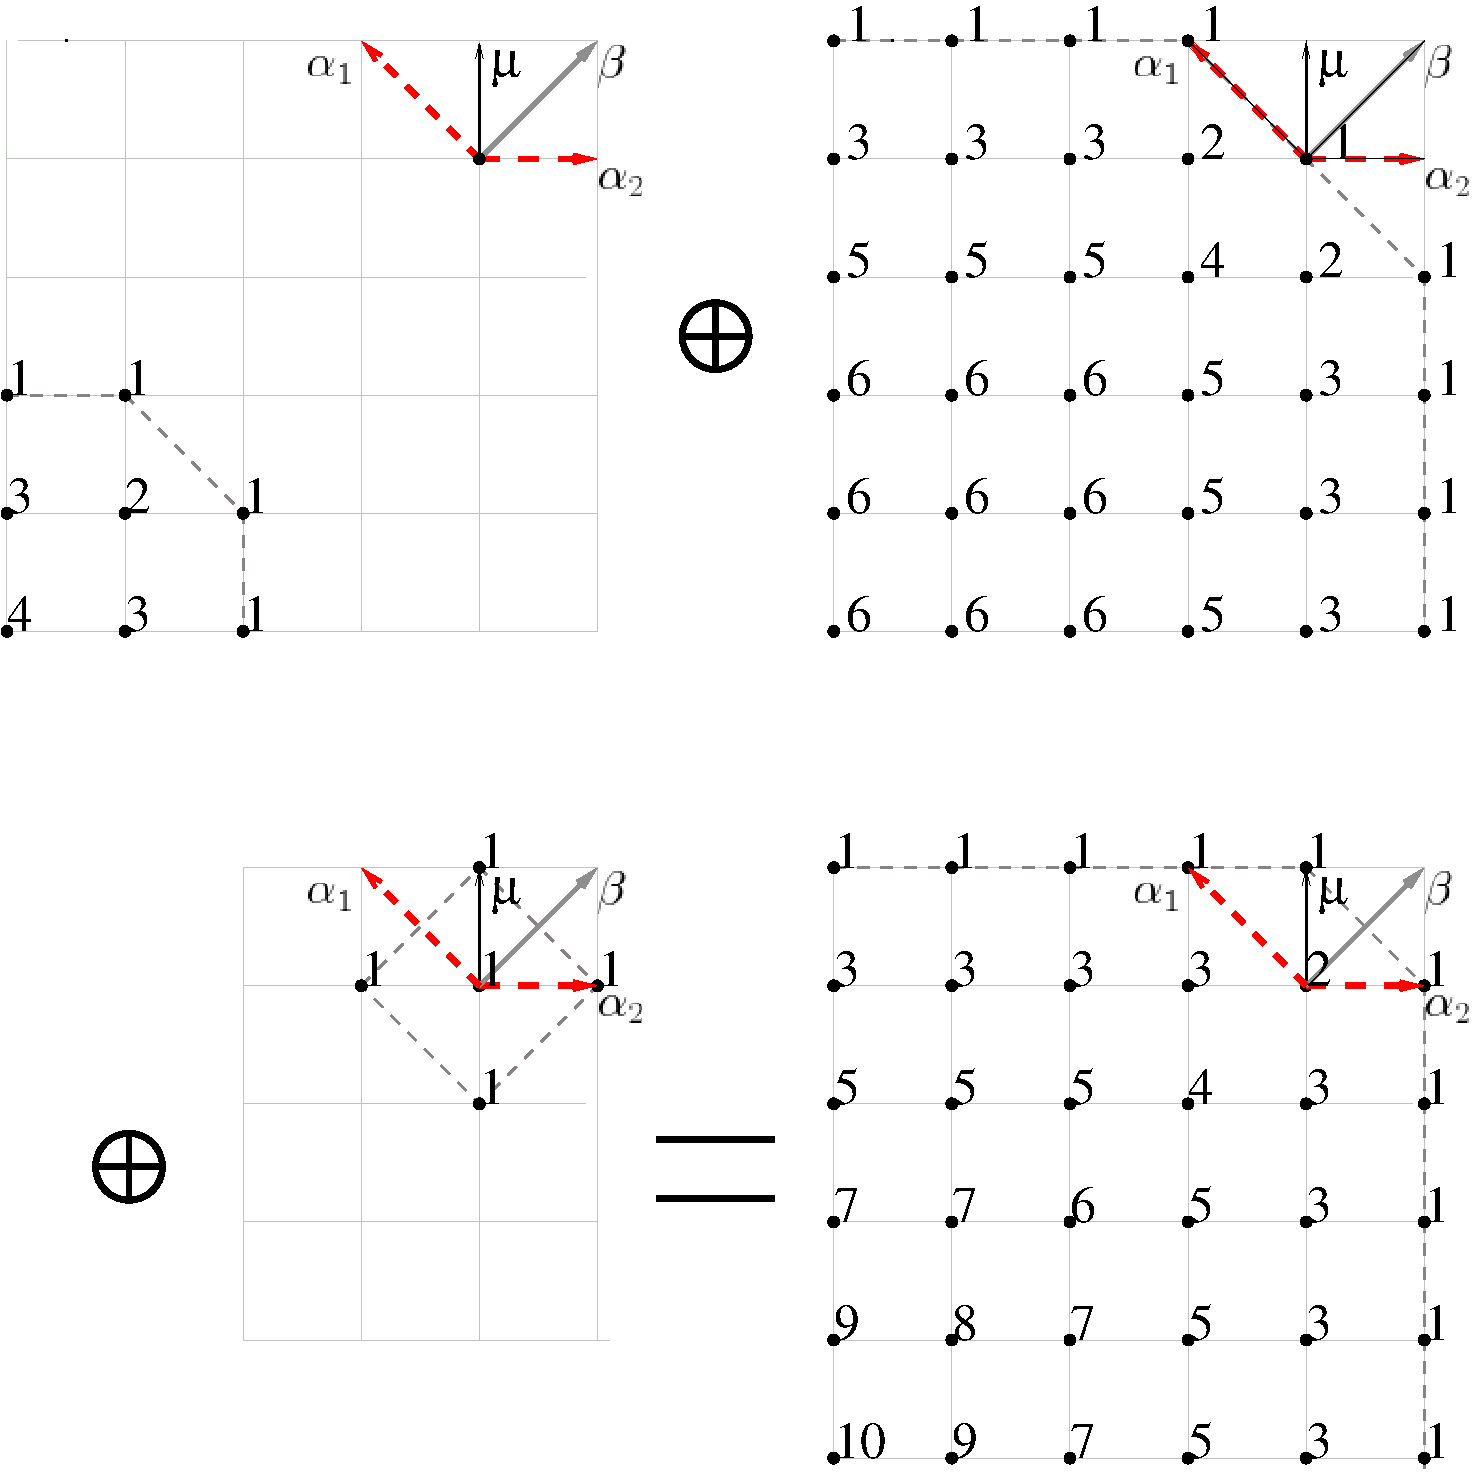
\includegraphics[width=140mm]{B2_Decomp}
 }
 \caption{Character decomposition of generalized Verma module $M^{\mu=\omega_{1}}_{I}$ to the
   characters of the irreducible modules. Simple roots $\alpha_1, \alpha_2$ of $B_2$ are presented as the dashed vectors.
    The simple root $\beta = \alpha_1+2\alpha_2$ of $A_1$ is indicated as the grey vector. The
    highest weight $\mu$ is shown by the black arrow. }
\end{figure}


\begin{figure}[h!bt]
 \noindent\centering{
   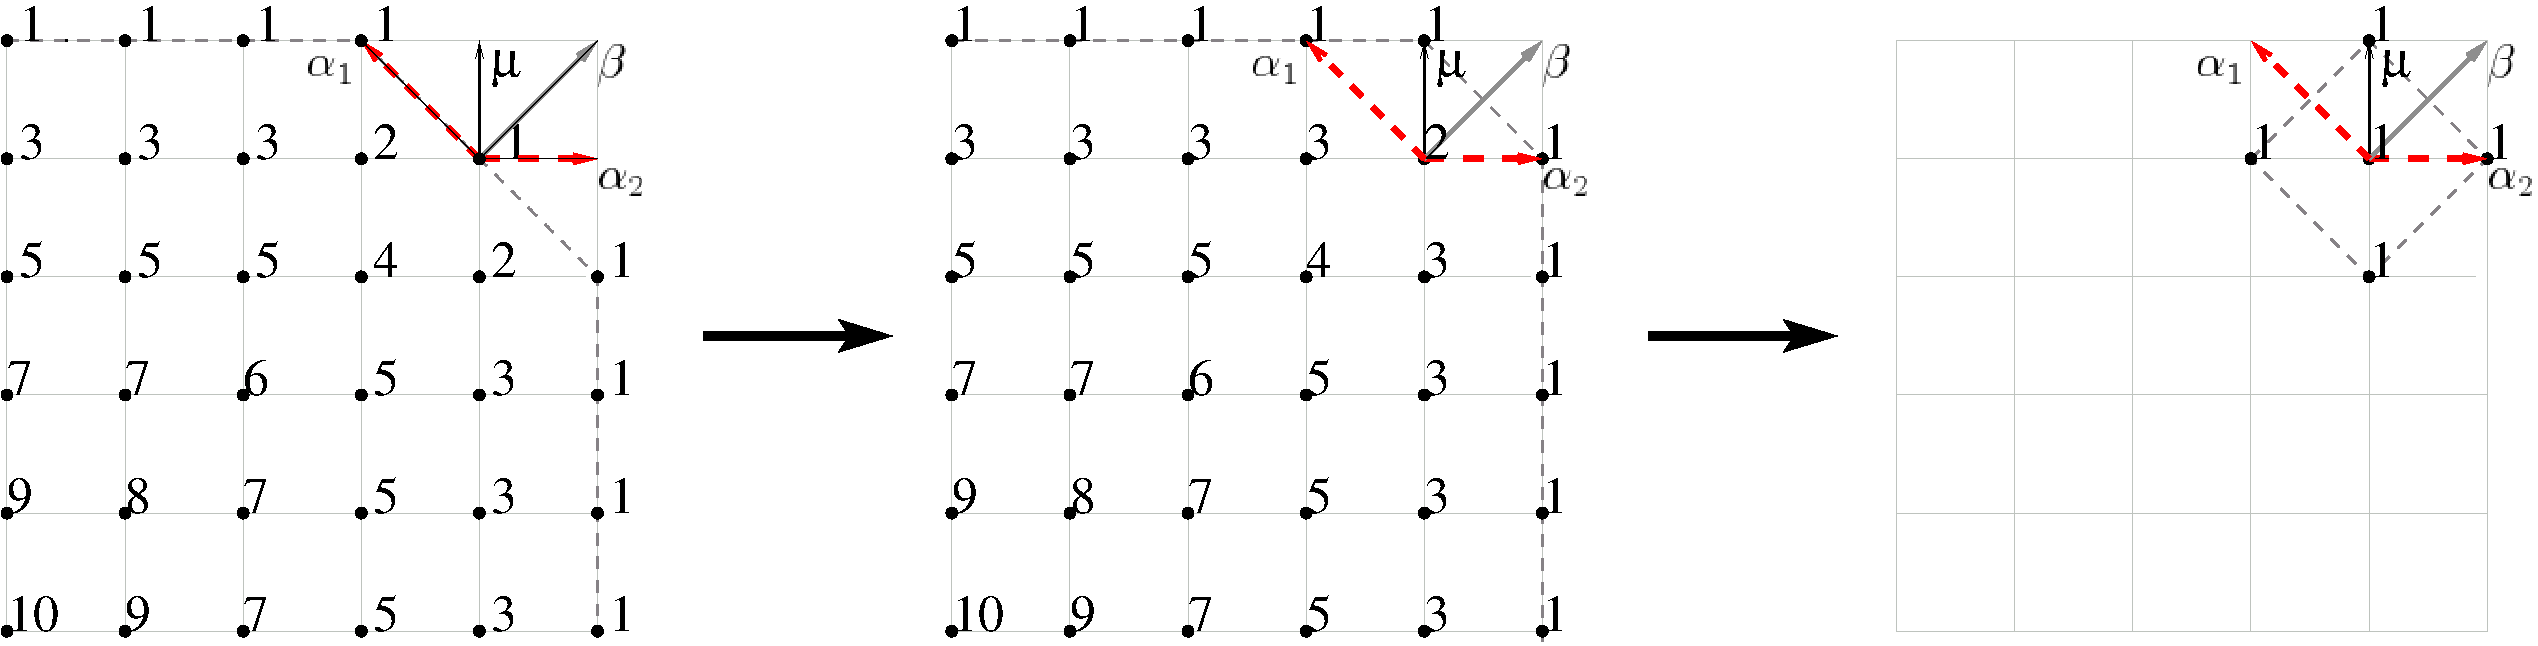
\includegraphics[width=140mm]{B2_Exact}}
 \caption{Part of the exact sequence
   $M_{I}^{\mu(u_{(1)})}/\left(M_{I}^{\mu(w_{(2)})}/M_{I}^{\mu(w_{(3)})}\right)\to M^{\mu}_{I}\to
   L^{\mu}\to 0 $ for Lie algebra $B_2$. Here $w_{(i)}\in  U$ is Weyl reflection of the length $i$, $\mu=\omega_{1}$.}

\end{figure}


%%  \begin{figure}[h!bt]
%%   \noindent\centering{
%%     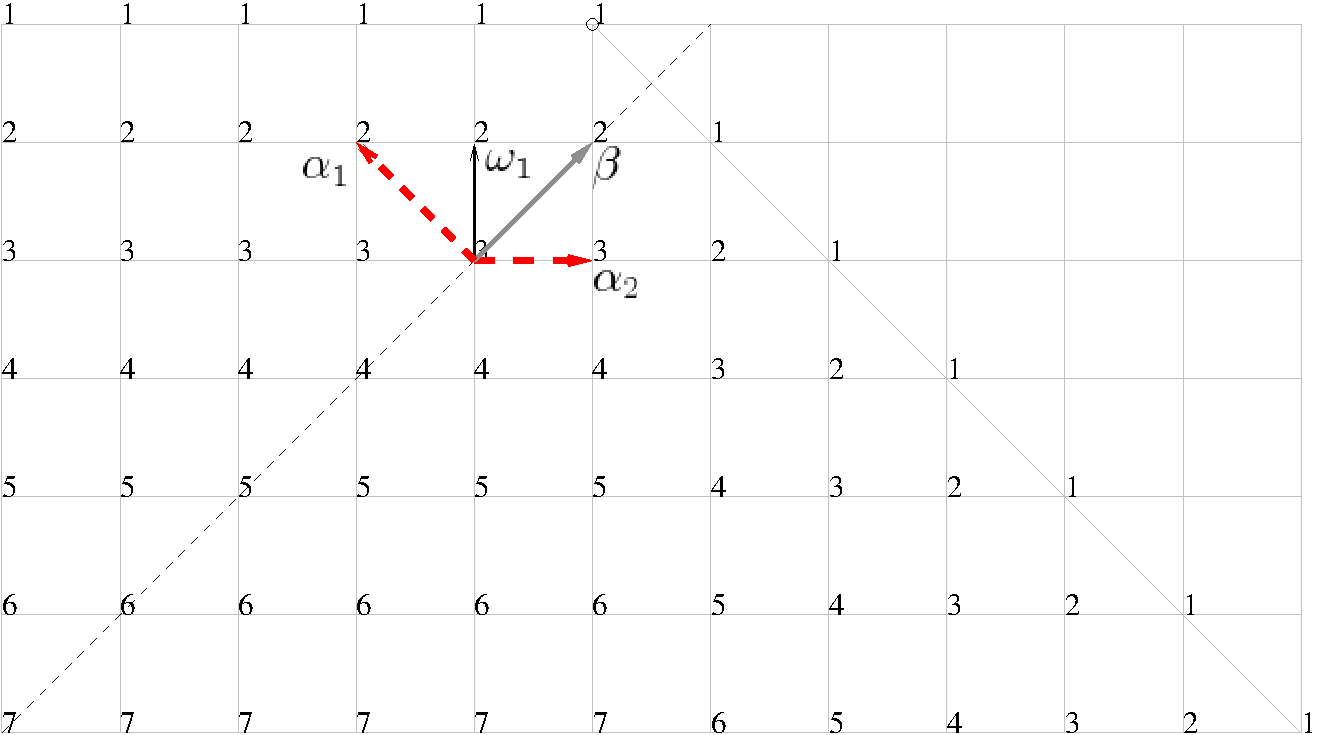
\includegraphics[width=120mm]{B2_Verma}
%%    }
%%   \caption{Regular embedding of $A_1$ into $B_2$. Simple roots $\alpha_1, \alpha_2$ of $B_2$ are presented as the dashed vectors.
%%      The simple root $\beta = \alpha_1+2\alpha_2$ of $A_1$ is indicated as the grey vector.
%%  Dimensions of weight subspaces of Verma module $M^{(1,2)}$ are shown.}
%%    \label{fig:B2_Verma}
%%  \end{figure}
%%  
The branching coefficients are shown at Figure \ref{fig:B2_Verma_Branch2}
for the regular embedding $A_{1}\rightarrow B_{2}$. Here we can
see that the picture depends upon the embedding and looks similar to the
Verma modules of some subalgebra.

%%  
%%  \begin{figure}[h!bt]
%%    \noindent\centering{
%%     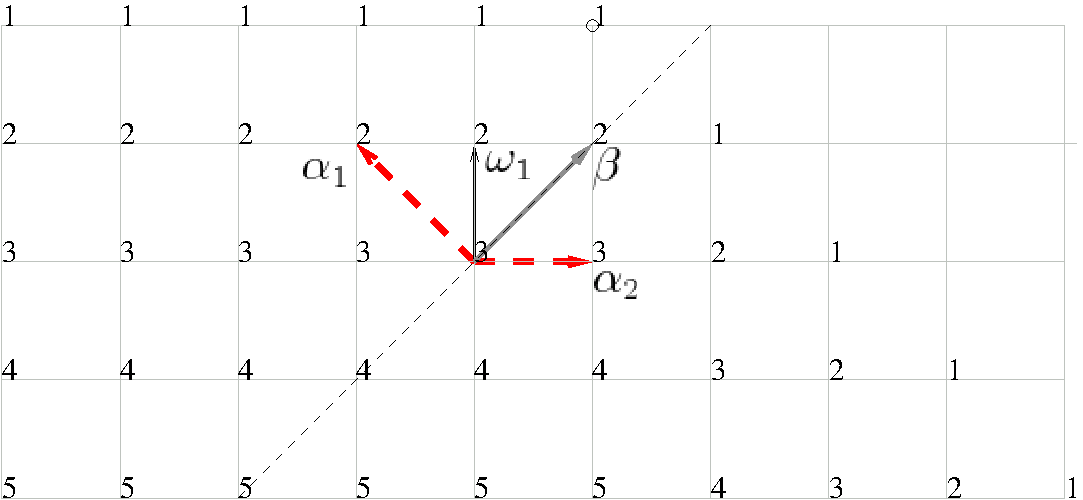
\includegraphics[width=120mm]{B2_Verma_Branch4.pdf}
%%    }
%%    \caption{Branching of the Verma module $M^{(1,2)}$ for the regular embedding of $A_1$ into $B_2$. Simple roots $\alpha_1, \alpha_2$ of $B_2$ are presented as the dashed vectors.
%%      The simple root $\beta = \alpha_1+2\alpha_2$ of $A_1$ is indicated as the grey vector.
%%      Branching coefficients for Verma module of the subalgebra are shown. Dashed line indicates the
%%      direction of subalgebra modules.}
%%   \label{fig:B2_Verma_Branch2}
%%  \end{figure}
%%  
\end{example}
In the present paper we interpret this branching coefficients as the dimensions
of the weight subspaces of modules of contracted algebras.

\subsection{Weyl-Verma formulas.}

\begin{statement}
\bigskip For an orthogonal subalgebra $\afb$ in $\gf$
(orthogonal partner of reductive $\af\hookrightarrow \gf$) the
character of an integrable highest weight module $L^{\mu }$ can be presented
as a combination (with integral coefficients) of parabolic Verma modules
distributed by the set of weights $e^{\mu _{\aft}\left( u\right) }$:
\begin{equation*}
\mathrm{ch}\left( L^{\mu }\right) =\sum_{u\in U}\;\epsilon (u)e^{\mu _{%
\widetilde{\af}}\left( u\right) }\mathrm{ch}M_{I}^{\mu _{\af%
_{\perp }}\left( u\right) },
\end{equation*}
where $U:=\left\{ u\in W|\quad \mu _{\afb}\left( u\right) \in
\overline{C_{\afb}}\right\} $ and $\Delta _{I}^{+}$ is
equivalent to $\Delta _{\afb}^{+}$.
\end{statement}

\bigskip
\begin{proof}
By the definition (\ref{delta a ort}) the subalgebra $%
\mathfrak{a}_{\bot }$ is regular and reductive. Consider its Weyl
denominator $R_{\afb}:=\prod_{\alpha \in \Delta _{\af%
_{\perp }}^{+}}\left( 1-e^{-\alpha }\right) ^{\mathrm{mult}_{\af}%
\mathrm{\left( \alpha \right) }}$ and the element $R_{J}:=\prod_{\alpha \in
\Delta ^{+}\setminus \Delta _{\afb}^{+}}\left( 1-e^{-\alpha
}\right) ^{\mathrm{mult}(\alpha )}$ as the factors in $R$: $\quad $%
\begin{equation*}
R=R_{J}R_{\afb}.
\end{equation*}
According to this factorization and the decomposition (\ref{sing decomp main}%
) the character $\mathrm{ch}\left( L^{\mu }\right) $ can be written as
\begin{eqnarray*}
\mathrm{ch}\left( L^{\mu }\right) &=&\left( R_{J}\right) ^{-1}\left( R_{%
\afb}\right) ^{-1}\Psi ^{\mu }=\left( R_{J}\right)
^{-1}\sum_{u\in U}\;e^{\mu _{\widetilde{\af}}\left( u\right) }\epsilon
(u)\left( R_{\afb}\right) ^{-1}\Psi _{\afb}^{\mu _{%
\afb}\left( u\right) } \\
&=&\left( R_{J}\right) ^{-1}\sum_{u\in U}\;e^{\mu _{\widetilde{\af}%
}\left( u\right) }\epsilon (u)L_{\afb}^{\mu _{\afb}\left( u\right) },
\end{eqnarray*}
where $\left\{ L_{\afb}^{\mu _{\afb}\left(
u\right) }|u\in U\right\} $ is the set of finite-dimensional $\af%
_{\perp }$-modules with the highest weights $\mu _{\afb}\left(
u\right) $. We are interested in nontrivial subalgebras $\af$ and
correspondingly in nontrivial $\afb$ (the case of a trivial
orthogonal subalgebra arise when $\af=\gf$ and was considered
above (see Remark 1)). This means that $r_{\af}\geq 1$ and $r_{\af%
_{\perp }}<r$. Due to the fact that any maximal regular subalgebra has the
Dynkin scheme obtained by one or two node subtractions from the extended
Dynkin scheme and the extended scheme has at most one dependent root (the
highest root) the set of roots $\Delta _{\afb}^{+}$ is always
equivalent to the one $\Delta _{I}^{+}$ generated\ by some subset $I\subset
S $ of simple roots.

It follows that we can (by redefining the set $\Delta ^{+}$) identify $%
\Delta _{\afb}^{+}$ with the subset $\Delta _{I}^{+}$ \ where $%
I\subset S$ . This allows us to introduce the elements necessary to compose
the generalized Verma modules
\cite{lepowsky1977generalization,humphreys2008representations}.
We have two sets of root
vectors $\left\{ x_{\xi }\in \gf_{\xi }|\xi \in \Delta _{I}^{+}\right\}
$ and $\left\{ x_{\eta }\in \gf_{\eta }|\eta \in \Delta ^{+}\setminus
\Delta _{I}^{+}\right\} $. They generate nilpotent subalgebras of $\frak{n}%
^{+}$:
\begin{equation*}
\frak{n}_{I}^{+}:=\sum_{\xi \in \Delta _{I}^{+}}\gf_{\xi },\quad
\frak{u}_{I}^{+}:=\sum_{\eta \in \Delta ^{+}\setminus \Delta _{I}^{+}}\gf%
_{\eta }.
\end{equation*}
The first subalgebra together with its negative counterpart $\frak{n}%
_{I}^{-} $ generates a simple subalgebra
\begin{equation*}
\frak{s}_{I}=\frak{n}_{I}^{-}+\frak{h}_{I}+\frak{n}_{I}^{+}.
\end{equation*}
We enlarge it with the remaining Cartan generators and introduce the
subalgebra:
\begin{equation*}
\frak{l}_{I}=\frak{n}_{I}^{-}+\frak{h}+\frak{n}_{I}^{+}.
\end{equation*}
The semidirect product of subalgebras $\frak{l}_{I}$ and $\frak{u}_{I}^{+}$
gives a parabolic subalgebra $\frak{p}_{I}\hookrightarrow \gf$ :
\begin{equation}
\frak{p}_{I}=\frak{l}_{I}\vartriangleright \frak{u}_{I}^{+},
\label{paralolic subalg}
\end{equation}
Its universal enveloping $U\left( \frak{p}_{I}\right) $ is a subalgebra in $%
U\left( \gf\right) $. According to the obtained structure (\ref
{paralolic subalg}) the $\frak{l}_{I}$-modules $L_{\afb}^{\mu _{%
\afb}\left( u\right) }$ can be easily lifted to $\frak{p}_{I}$%
-modules using the trivial action of the nilradical $\frak{u}_{I}^{+}$. The
latter induce $U\left( \gf\right) $-modules in a standard way:
\begin{equation*}
M_{I}^{\mu _{\afb}\left( u\right) }=U\left( \gf\right)
\otimes _{U\left( \frak{p}_{I}\right) }L_{\afb}^{\mu _{\af%
_{\perp }}\left( u\right) }.
\end{equation*}
According to the defenition presented in \cite{lepowsky1977generalization}
these are the \textit{generalized Verma modules}
generated by the highest weights $\mu _{\af%
_{\perp }}\left( u\right) $. As a $U\left( \frak{u}_{I}^{-}\right) $-module
each $M_{I}^{\mu _{\afb}\left( u\right) }$ is isomorphic to $%
U\left( \frak{u}_{I}^{-}\right) \otimes $ $L_{\afb}^{\mu _{%
\afb}\left( u\right) }$ and thus its character can be written
with the help of Kostant-Heckman function \cite{KostantHeckman1982} corresponding
to the injection of the orthogonal subalgebra $\afb\hookrightarrow \gf$:
\begin{equation*}
\mathrm{ch}M_{I}^{\mu _{\afb}\left( u\right) }=\mathcal{KH}_{%
\afb\hookrightarrow \gf}\mathrm{ch}L_{\afb}^{\mu _{\afb}\left( u\right) }.
\end{equation*}
As far as the function $\mathcal{KH}_{\afb\hookrightarrow \frak{%
g}}$ is generated by the denominator $R_{I}$ the last expression can be
rewritten in the form
\begin{equation*}
\mathrm{ch}M_{I}^{\mu _{\afb}\left( u\right) }=\frac{1}{R_{I}}%
\mathrm{ch}L_{\afb}^{\mu _{\afb}\left( u\right) }.
\end{equation*}
This means that we have obtained the generalized Weyl-Verma character formula
-- the decomposition of $\mathrm{ch}\left(
L^{\mu }\right) $ in terms of generalized Verma modules characters:
\begin{equation}
\mathrm{ch}\left( L^{\mu }\right) =\sum_{u\in U}\;e^{\mu _{\aft}\left(
u\right) }\epsilon (u)\mathrm{ch}M_{I}^{\mu _{\afb}\left(
u\right) }.  \label{char in gen verma mod}
\end{equation}
\end{proof}

\begin{remark}
Here the generalized Weyl-Verma character formula appear in a detailed
form: the weights $\mu _{\aft}$ and the generalized Verma modules highest weights
$\mu _{\afb}$ are indicated separately. The reason is that the
highest weight of $M_{I}$-module is not equal to the projection of the maximal
weight to $h^*_{\afb}$ (but must be additionally shifted by the defect).
\end{remark}

\begin{example}
  Continuing Example \ref{example:reduct-verma-modul} we consider the generalized Verma modules for the
  embedding  $A_{1}\hookrightarrow B_{2}$ with the subalgebra $\afb$ built on the root $\alpha_{1}$
  of $B_{2}$. The generalized Verma module $M^{\omega_{1}}_{I}$ with the highest weight
  $\omega_{1}=e_{1}$ is shown in Figure \ref{fig:B2_Verma_Decomp}. The decomposition of the corresponding irreducible module
  $L^{\omega_{1}}$ is indicated by the set of dashed contours of the involved generalized Verma
  modules. 
%%     \begin{figure}[h!bt]
%%    \noindent\centering{
%%     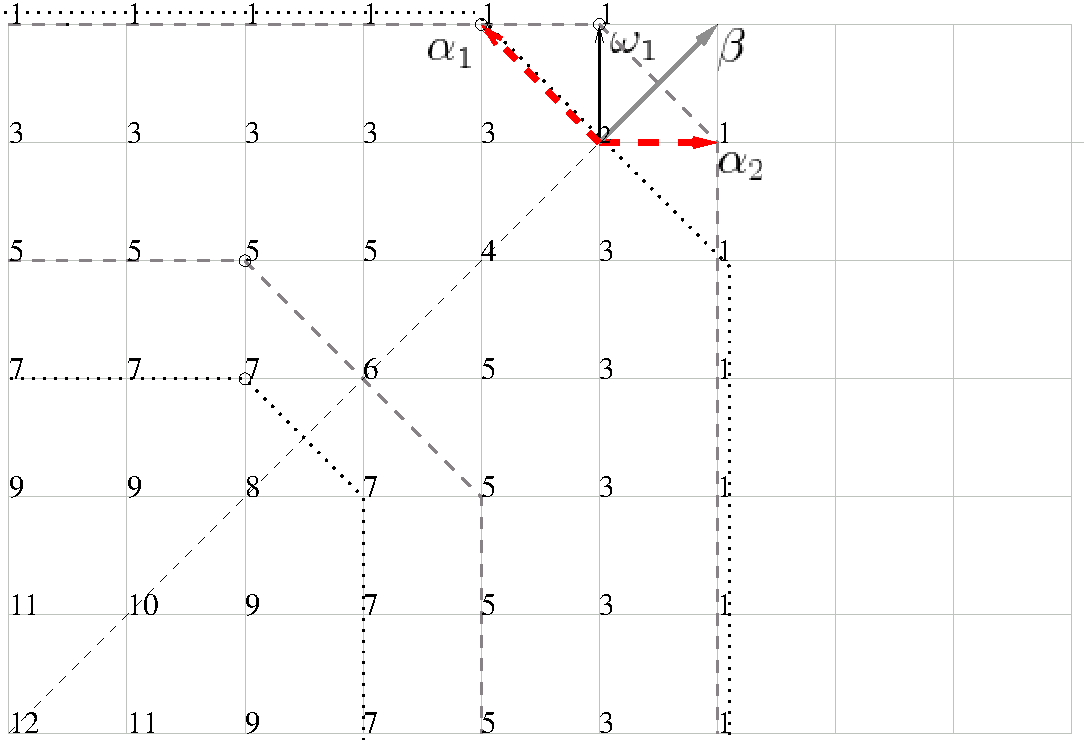
\includegraphics[width=120mm]{B2_Gen_Verma_Decomp}
%%    }
%%    \caption{Generalized Verma module  for the regular embedding of $A_1$ into $B_2$. Simple roots $\alpha_1, \alpha_2$ of $B_2$ are presented as the dashed vectors.
%%      The simple root $\beta = \alpha_1+2\alpha_2$ of $A_1$ is indicated as the grey vector. The
%%      decomposition of $L^{\omega_{1}}$ is indicated by the set of dashed contours of the involved generalized Verma
%%    modules. Dashed contours correspond to positive $\epsilon(u)$ and dotted to negative.}
%%  
%%   \label{fig:B2_Verma_Decomp}
%%  \end{figure}

\end{example}

\begin{remark}
As it was proved in \cite{humphreys2008representations} (see Proposition 9.6 ) the characters of the
generalized Verma modules $M_{I}^{\mu _{\afb}\left( u\right) }$
can be described as linear combinations of ordinary Verma modules of $\frak{g%
}$:
\begin{equation*}
\mathrm{ch}M_{I}^{\mu _{\afb}\left( u\right) }=\sum_{w\in W_{%
\afb}}\epsilon \left( w\right) \mathrm{ch}M^{w\left( \mu _{%
\afb}\left( u\right) +\rho _{\afb}\right) -\rho _{%
\afb}}
\end{equation*}
Substituting this expression in\ (\ref{char in gen verma mod}) and using the
definitions (\ref{mu-a},\ref{mu-a-tilda}) and (\ref{defect ort}) we reobtain
the standard Weyl-Verma decomposition of the character:
\begin{equation*}
\mathrm{ch}\left( L^{\mu }\right) =\sum_{w\in W}\;\epsilon (u)\mathrm{ch}%
M^{w\left( \mu +\rho \right) -\rho }.
\end{equation*}
\end{remark}

%\bigskip



\section{Conclusions}

\label{sec:conclusions}


In \cite{2010arXiv1007.0318L} it was demonstrated that the injection fan recursive mechanism
works also for special injections. Here we must stress that the Weyl-Verma decomposition
can be obtained in this case. The Weyl-Verma relations corresponding to the special
subalgebras will describe the projections of characters of the initial module in terms
of generalized Verma modules distributed in the subspace of $h^*$.


Consider the situation where the simple roots are prescribed by some external
forces (originating in physical applications conditions, for example). In this case
the orthogonal partner cannot be generated by simple root vectors only.  The elements
$\frak{u}_{I}^{+}:=\sum_{\eta \in \Delta ^{+}\setminus \Delta _{I}^{+}}\gf%
_{\eta }$ do not form a subalgebra in $\gf$ because some nonsimple roots are lost in
$\Delta ^{+}\setminus \Delta _{I}^{+}$. It is important to indicate that in this case
the Weyl-Verma formula still exists. In it the generalized Verma modules correspond to
the contractions \cite{Doebner1967Melsheimer} of the algebra $\frak{n}^{+}$ and the
Weyl-Verma relations describes the decomposition of the representation space of $L^{\mu}$
into the set of generalized Verma modules of contracted algebra
$U\left(\frak{n}_c^{+}\right)$. The weight vectors are formed by the PBW-basis
of $U\left(\frak{n}_c^{+}\right)$ and of $U\left( \afb \right)$. To consider such space
as a $\gf$-module we must perform the deformation \cite{Nijenhuis1966Richardson} of
the algebra $\frak{n}_c^{+}$ (restore the initial composition law). The space survives
and after such a deformation the initial
algebra generators will act properly on it.



\section{Acknowledgments}
The authors express their sincere gratitude to all those who prepared and performed the
III International Conference "Models in Quantum Field Theory - 2010" dedicated to 70-th
anniversary of A. N. Vassiliev.

The work was supported in part by the RFFI grant N 09-01-00504.

% \section{Applications}
% \label{sec:applications}
%
% \section{Conclusion}
% \label{sec:conclusion}
%
%
% \section{Acknowledgements}
%
% The work was supported in part by RFFI grant N 09-01-00504 and the National
% Project RNP.2.1.1./1575.
%



\bibliographystyle{utphys}
\bibliography{article}
{}


\end{document}
